\subsection*{Partie A}
\begin{enumerate}
\item La fonction $f:x \mapsto \dfrac{x-2}{2x-3}$ est dérivable sur $]-\infty~;~\frac32[$ en tant que quotient de fonctions polynomiales, le dénominateur étant non nul. On a :

\[\begin{array}{rcl}
f'(x) &=& \dfrac{1 \times (2x - 3) - (x - 2) \times 2}{(2x - 3)^2} \\
&=& \dfrac{2x - 3 - 2x + 4}{(2x - 3)^2}\\
&=& \dfrac{1}{(2x - 3)^2}
\end{array}\]

Pour tout $x \in \left]-\infty~;~\frac32\right[$,\: $(2x - 3)^2 > 0$, donc $f'(x) > 0$. La fonction $f$ est strictement croissante sur l'intervalle $\left]-\infty~;~\frac32\right[$.

Étudions les limites de $f$ aux bornes de son ensemble de définition :
\begin{itemize}
	\item Limite en $-\infty$: 
	\[\begin{matrix}
	f(x) &=&\dfrac{x-2}{2x-3} \\
	&=&\dfrac{x\left(1-\dfrac2{x}\right)}{x\left(2-\dfrac3{x}\right)}\\
	& =&\dfrac{1-\frac2{x}}{2-\frac3{x}}, \\
\end{matrix}\]

donc puisque $\displaystyle \lim_{x \to - \infty}\dfrac2{x} = \displaystyle \lim_{x \to - \infty}\dfrac3{x} = 0$, on en déduit que $\displaystyle \lim_{x \to - \infty} f(x)  = \dfrac12$ \text{(quotient de limites)}

\item Limite en $\frac{3}{2}, \: x < \frac{3}{2}$: 
\[ 
\left.
\begin{matrix}
\displaystyle \lim_{\substack{x \to \frac32\\ x < \frac32}}x - 2 &=& -\frac12 \\
\displaystyle \lim_{\substack{x \to \frac32\\ x < \frac32}} 2x-3 &=& 0^-
\end{matrix}
\right\}
\Rightarrow \lim_{\substack{x \to \frac32\\ x < \frac32}} f(x)= +\infty \text{ (quotient de limites)} 
\]
\end{itemize}
On en déduit donc le tableau de variations suivant:

\begin{center}
\begin{tikzpicture}
\tkzTabInit{$x$ / 1 , $f'(x)$ / 1 , $f$ / 2}{$-\infty$, $\frac32$}
\tkzTabLine{, +, d}
\tkzTabVar{-/ $\frac12$, +D/ $+\infty$}
\end{tikzpicture}
\end{center}

\item Sur l'intervalle $[- \infty~;~\frac32]$, donc a fortiori sur l'intervalle [0~;~1] la fonction $f$ est strictement croissante. Ainsi :

\[\begin{array}{rcl}
0 \leqslant x \leqslant 1 &\implies& f(0) \leqslant f(x) \leqslant f(1) \\
&\implies& \dfrac{-2}{-3} \leqslant f(x) \leqslant \dfrac{-1}{-1} \\
&\implies& \dfrac{2}{3} \leqslant f(x) \leqslant 1
\end{array}\]

Puisque $\frac{2}{3} \geqslant 0$, on en déduit que pour tout $x \in [0~;~1]$,\: $f(x) \in [0~;~1]$.
\end{enumerate}

\medskip

\subsection*{Partie B}
\begin{enumerate}
\item Démontrons par récurrence que pour tout entier naturel $n$, $0 \leqslant u_n \leqslant u_{n+1} \leqslant 1$.
\begin{itemize}
\item \textbf{Initialisation :} Pour $n = 0$, on a $u_0 = 0$ et $u_1 = f(0) = \frac{2}{3}$. On a bien $0 \leqslant 0 \leqslant \frac{2}{3} \leqslant 1$, soit $0 \leqslant u_0 \leqslant u_1 \leqslant 1$. La propriété est initialisée.
\item \textbf{Hérédité :} Soit $n \in \N$, tel que $0 \leqslant u_n \leqslant u_{n+1} \leqslant 1$

La fonction $f$ étant strictement croissante sur $[0~;~1]$, elle conserve l'ordre, on a donc:

\[\begin{array}{rl}
& 0 \leqslant u_n \leqslant u_{n+1} \leqslant 1 \\
\implies & f(0) \leqslant f(u_n) \leqslant f(u_{n+1}) \leqslant f(1) \\
\implies & \frac{2}{3} \leqslant u_{n+1} \leqslant u_{n+2} \leqslant 1
\end{array}
\]
Comme $0 \leqslant \frac{2}{3}$, on obtient $0 \leqslant u_{n+1} \leqslant u_{n+2} \leqslant 1$. L'encadrement est vrai au rang $n + 1$.
\item \textbf{Conclusion :} L'encadrement est vrai au rang 0 et s'il est vrai à un rang supérieur ou égal à 0, il l'est aussi au rang suivant : par le principe de récurrence :

Pour tout entier naturel $n$, $0 \leqslant u_n \leqslant u_{n+1} \leqslant 1$.
\end{itemize}

\item Le résultat précédent montre :

-- que $u_n \leqslant u_{n+1}$ donc que la suite $(u_n)$ est croissante et 

-- majorée par 1 puisque tous ses termes le sont.

D'après le théorème de convergence monotone, la suite $(u_n)$ converge vers une limite réelle $\ell$ vérifiant $0 \leqslant \ell \leqslant 1$.

\item La fonction $f$ étant continue, la limite $\ell$ est solution de l'équation $f(x) = x$.

\[\begin{array}{rcl}
\dfrac{x - 2}{2x - 3} = x &\iff& x - 2 = x(2x - 3) \\
&\iff& x - 2 = 2x^2 - 3x \\
&\iff& 2x^2 - 4x + 2 = 0 \\
&\iff& 2(x - 1)^2 = 0 \\
&\iff& (x - 1)^2 = 0\\
&\iff& (x - 1) = 0\\
&\iff& x  = 1\\
\end{array}\]

On en déduit que $\ell = 1$ et donc que la suite $(u_n)$ converge vers 1.
\item La fonction \texttt{seuil(0.0001)} renvoie la plus petite valeur de l'entier $n$ telle que $u_n \geqslant 1 - \np{0,0001}$, c'est-à-dire $u_n \geqslant \np{0,9999}$. La valeur \np{5000} signifie que c'est à partir du rang $n = \np{5000}$ que les termes de la suite dépassent \np{0,9999}.

\item
\begin{enumerate}
\item Les premiers termes sont :

\[\begin{array}{rcl}
u_0 &=& 0 \\
u_1 &=& \frac{2}{3} \\
u_2 &=& \frac{\frac{2}{3} - 2}{2\left(\frac{2}{3}\right) - 3} = \frac{-\frac{4}{3}}{-\frac{5}{3}} = \frac{4}{5} \\
u_3 &=& \frac{\frac{4}{5} - 2}{2\left(\frac{4}{5}\right) - 3} = \frac{-\frac{6}{5}}{-\frac{7}{5}} = \frac{6}{7}
\end{array}\]

\item On peut conjecturer que $u_n = \dfrac{2n}{2n + 1}$.

Démontrons-le par récurrence :

\begin{itemize}
\item \textbf{Initialisation :} Pour $n = 0$, $\frac{2 \times 0}{2 \times0 + 1} = \frac01 = 0 = u_0$. La propriété est vraie au rang 0.
\item \textbf{Hérédité :} Soit $n \in \N$, tel que $u_n = \frac{2n}{2n + 1}$.

\[\begin{array}{rcl}
u_{n+1} &=& f(u_n) = \frac{\frac{2n}{2n+1} - 2}{2\left(\frac{2n}{2n+1}\right) - 3} \\
&=& \frac{\frac{2n - 2(2n+1)}{2n+1}}{\frac{4n - 3(2n+1)}{2n+1}} \\
&=& \frac{2n - 4n - 2}{4n - 6n - 3} \\
&=& \frac{-2n- 2}{-2n - 3} \\&=& \frac{2n+2}{2n+3}\\
&=& \frac{2n+2}{2n+2 + 1}\\
u_{n+1} &=&\dfrac{2(n+1)}{2(n+1) + 1}\\
\end{array}\]

La relation est vraie au rang $n + 1$.
\item La relation est vraie au rang 0 et si elle est vraie au rang $n \geqslant 0$, elle l'est aussi au rang $n + 1$. Par le principe de récurrence on a donc montré que:

\[\text{quel que soit}\: n \in \N,\enskip u_n=\frac{2n}{2n+1}\]
\end{itemize}
	\end{enumerate}
\end{enumerate}
